\begin{frame}
	\myheading{Module 5.9 : Gradient Descent with Adaptive Learning Rate}
\end{frame}

\begin{frame}
	
	\begin{columns}
		
		\column{0.25\textwidth}
		\begin{overlayarea}{\textwidth}{\textheight}
			\begin{tikzpicture}
\begin{axis}[axis lines=left, ticks=none,xmax=0.5,ymax=0.5,x label style={at={(axis description cs:0.5,0)},anchor=north},
xlabel={$\theta$}, ylabel={error}]
\addplot[thick,black, no markers, samples=200, domain=-5:0] {-x*exp(x)};
\only<2->{\draw[dashed] (axis cs:-1.88,0.31) -- (axis cs:-0.0,0.31)} ;
\only<2->{\draw[dashed] (axis cs:-2.68,0.21) -- (axis cs:-0.0,0.21)} ;

\end{axis}
\end{tikzpicture}

		\end{overlayarea}
		
		\column{0.75\textwidth}
		
		\begin{overlayarea}{\textwidth}{\textheight}
			\begin{itemize}\justifying
				\item<2->{Given this network, it should be easy to see that given a single point ($\mathbf{x}, y$)...}  
				\item<3->{$\nabla w^1 = (f(\mathbf{x}) - y) * f(\mathbf{x}) * (1- f(\mathbf{x})) * x^1$ } 
				\item<3->{$\nabla w^2 = (f(\mathbf{x}) - y) * f(\mathbf{x}) * (1- f(\mathbf{x})) * x^2$ }... so on  
				\item<4-> If there are $n$ points, we can just sum the gradients over all the $n$ points to get the total gradient
				\item<5-> What happens if the feature $x^2$ is very sparse? \onslide<6->{(\textit{i.e.}, if its value is 0 for most inputs)}  
				\item<7-> $\nabla w^2$ will be 0 for most inputs (see formula) and hence $w^2$ will not get enough updates
				\item<8-> If $x^2$ happens to be sparse as well as important we would want to take the updates to $w^2$ more seriously
				\item<9-> Can we have a different learning rate for each parameter which takes care of the frequency of features ?
			\end{itemize}
		\end{overlayarea}
	\end{columns}
\end{frame}

\begin{frame}
	
	\begin{overlayarea}{\textwidth}{\textheight}
		\vspace{-0.2in}
		\begin{block}{Intuition}
			\begin{itemize}\justifying
				\item<1-> Decay the learning rate for parameters in proportion to their update history \onslide<2->{(more updates means more decay)}
			\end{itemize}
		\end{block}
		
		\onslide<3->{
			\vspace{-0.1in}
			\begin{block}{Update rule for Adagrad}
				\begin{align*}
					v_t     & = v_{t-1} + {(\nabla w_{t})}^2                                \\
					w_{t+1} & = w_{t} - \frac{\eta}{\sqrt{v_{t} + \epsilon}} * \nabla w_{t} 
					\intertext{... and a similar set of equations for $b_t$}      
				\end{align*}
				
			\end{block}
		}
	\end{overlayarea}
\end{frame}

\begin{frame}
	\begin{columns}
		\column{0.6\textwidth}
		\begin{overlayarea}{\textwidth}{\textheight}
			\begin{itemize}\justifying
				\item<1-> To see this in action we need to first create some data where one of the features is sparse
				\item<2-> How would we do this in our toy network ? \onslide<3->{Take some time to think about it}
				\item<4-> Well, our network has just two parameters ($w$ and $b$). \onslide<5->{Of these, the input/feature corresponding to $b$ is always on} \onslide<6->{(so can't really make it sparse)}
				\item<7-> The only option is to make $x$ sparse
				\item<8-> \textbf{Solution:} We created $100$ random $(x,y)$ pairs and then for roughly $80\%$ of these pairs we set $x$ to 0 \onslide<9->{thereby, making the feature for $w$ sparse}
			\end{itemize}
		\end{overlayarea}
		
		\column{0.4\textwidth}
		\begin{overlayarea}{\textwidth}{\textheight}
			\begin{figure}
				\includegraphics<1->[scale=0.3]{images/module9/pseudo_code_adagrad_crop.png}
			\end{figure}
		\end{overlayarea}
	\end{columns}
\end{frame}


\begin{frame}
	\begin{columns}
		\column{0.65\textwidth}
		\begin{overlayarea}{\textwidth}{\textheight}
			\begin{itemize}\justifying
				\item<1-> GD (black), momentum (red) and NAG (blue)
				\item<2-> There is something interesting that these 3 algorithms are doing for this dataset. \onslide<3->{Can you spot it?}
				\item<4-> Initially, all three algorithms are moving mainly along the vertical ($b$) axis and there is very little movement along the horizontal ($w$) axis 
				\item<5-> Why? \onslide<6->{Because in our data, the feature corresponding to $w$ is sparse and hence $w$ undergoes very few updates} \onslide<7->{...on the other hand $b$ is very dense and undergoes many updates}
				\item<8-> Such sparsity is very common in large neural networks containing $1000s$ of input features and hence we need to address it
			\end{itemize}
		\end{overlayarea}
		
		\column{0.35\textwidth}
		\begin{overlayarea}{\textwidth}{\textheight}
			\begin{figure}
%				\begin{tikzpicture}
%					\sbox0{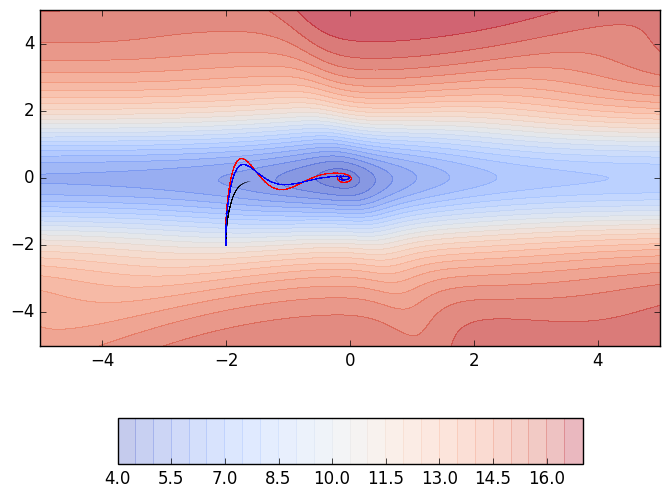
\includegraphics[scale=0.3]{images/module9/nag7/2d_path50.png}}% get width and height
%					\node[above right,inner sep=0pt] at (0,0)  {\usebox{0}};
%					\node[red,font=\small](w) at (0.5\wd0,0.23\ht0) {w};
%					\node[red,font=\small](b) at (0,0.67\ht0) {b};
%					\draw[->, line width=0.2mm](w)--(0.6\wd0,0.23\ht0);
%					\draw[->, line width=0.2mm](b)--(0,0.8\ht0);
%				\end{tikzpicture}
			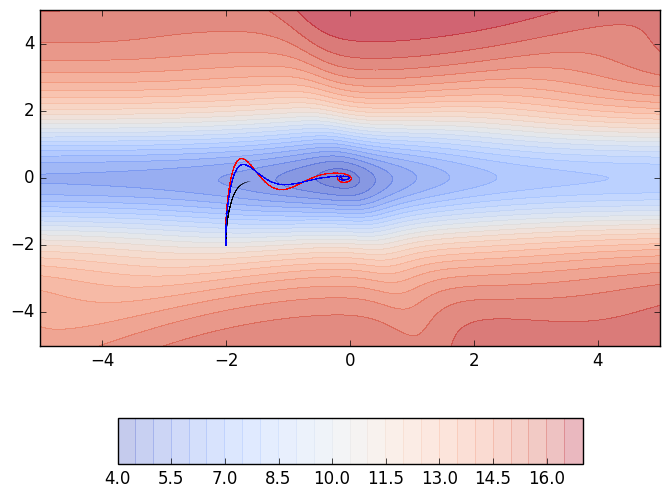
\includegraphics[scale=0.3]{images/module9/nag7/2d_path50.png}   
			\end{figure}
			\begin{itemize}\justifying
				\item<9-> Let's see what Adagrad does.... 
			\end{itemize}
			
		\end{overlayarea}
	\end{columns}
\end{frame}

\begin{frame}
	\begin{columns}
		\column{0.6\textwidth}
		\begin{overlayarea}{\textwidth}{\textheight}
			\begin{itemize}\justifying
				\item<91-> By using a parameter specific learning rate it ensures that despite sparsity $w$ gets a higher learning rate and hence larger updates
				\item<92-> Further, it also ensures that if $b$ undergoes a lot of updates its effective learning rate decreases because of the growing denominator
				\item<93-> In practice, this does not work so well if we remove the square root from the denominator \only<94->{(something to ponder about)}
				\item<95-> What's the flipside? \onslide<96->{over time the effective learning rate for $b$ will decay to an extent that there will be no further updates to $b$}
				\item<97-> Can we avoid this?  
			\end{itemize}
		\end{overlayarea}
		
		\column{0.4\textwidth}
		\begin{overlayarea}{\textwidth}{\textheight}
			
			\begin{figure}
				\foreach \n in {0,...,90} {%
%					\begin{tikzpicture}
%						\sbox0{\includegraphics[scale=0.35]{images/module9/adagrad7/2d_path\n.png}}% get width and height
%						\only<\n>{\node[above right,inner sep=0pt] at (0,0)  {\usebox{0}}};
%						\only<\n>{\node[red,font=\small](w) at (0.5\wd0,0.23\ht0) {w}};
%						\only<\n>{\node[red,font=\small](b) at (0,0.67\ht0) {b}};
%						\only<\n>{\draw[->, line width=0.2mm](w)--(0.6\wd0,0.23\ht0)};
%						\only<\n>{\draw[->, line width=0.2mm](b)--(0,0.8\ht0)};
%					\end{tikzpicture}
%				\pgfmathtruncatemacro\result{int(round(\n * 2))}
				\only<\n>{ \includegraphics[scale=0.35]{images/module9/adagrad7/2d_path\n.png}}%
				}%
				\only<91->{ 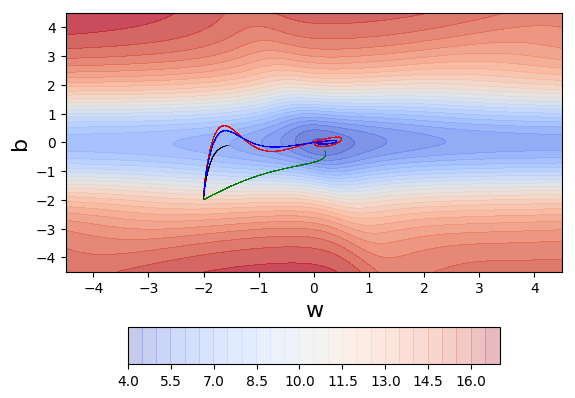
\includegraphics[scale=0.35]{images/module9/adagrad7/2d_path100.png}}
			\end{figure}
		\end{overlayarea}
	\end{columns}
\end{frame}


\begin{frame}
	\begin{overlayarea}{\textwidth}{\textheight}
		\vspace{-0.2in}
		\begin{block}{Intuition}
			\begin{itemize}\justifying
				\item<1-> Adagrad decays the learning rate very aggressively (as the denominator grows)
				\item<2-> As a result after a while the frequent parameters will start receiving very small updates because of the decayed learning rate
				\item<3-> To avoid this why not decay the denominator and prevent its rapid growth
			\end{itemize}
		\end{block}
		
		\only<4->{
			\begin{block}{Update rule for RMSProp}
				\begin{align*}
					v_t     & = \beta * v_{t-1} + (1 - \beta) {(\nabla w_{t})}^2            \\
					w_{t+1} & = w_{t} - \frac{\eta}{\sqrt{v_{t} + \epsilon}} * \nabla w_{t} 
					\intertext{... and a similar set of equations for $b_t$}      
				\end{align*}
				
			\end{block}
		}
	\end{overlayarea}
\end{frame}

\begin{frame}
	\begin{columns}
		\column{0.5\textwidth}
		\begin{overlayarea}{\textwidth}{\textheight}
			
			\begin{figure}
				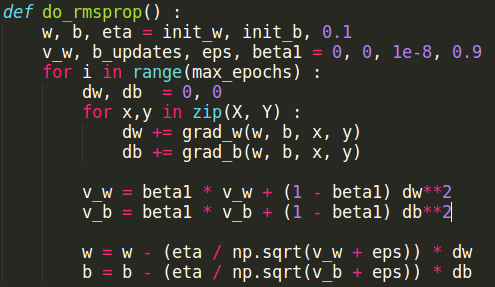
\includegraphics[scale=0.4]{images/module9/pseudo_code_rmsprop_crop.png}
			\end{figure}
			\onslide<60-> {\begin{itemize}\justifying
				\item {Adagrad got stuck when it was close to convergence} \onslide<30-> {(it was no longer able to move in the vertical ($b$) direction because of the decayed learning rate)}
				\end{itemize}}
		\end{overlayarea}
		
		\column{0.5\textwidth}
		\begin{overlayarea}{\textwidth}{\textheight}
			
			\begin{figure}
				\foreach \n in {0,...,60} {%
%					\begin{tikzpicture}
%						\sbox0{\includegraphics[scale=0.4]{images/module9/rmsprop7/2d_path\n.png}}% get width and height
%						\only<\n>{\node[above right,inner sep=0pt] at (0,0)  {\usebox{0}}};
%						\only<\n>{\node[red,font=\small](w) at (0.5\wd0,0.23\ht0) {w}};
%						\only<\n>{\node[red,font=\small](b) at (0,0.67\ht0) {b}};
%						\only<\n>{\draw[->, line width=0.2mm](w)--(0.6\wd0,0.23\ht0)};
%						\only<\n>{\draw[->, line width=0.2mm](b)--(0,0.8\ht0)};
%					\end{tikzpicture}
				\only<\n>{\includegraphics[scale=0.4]{images/module9/rmsprop7/2d_path\n.png}}%
				}
				\onslide<61->{
				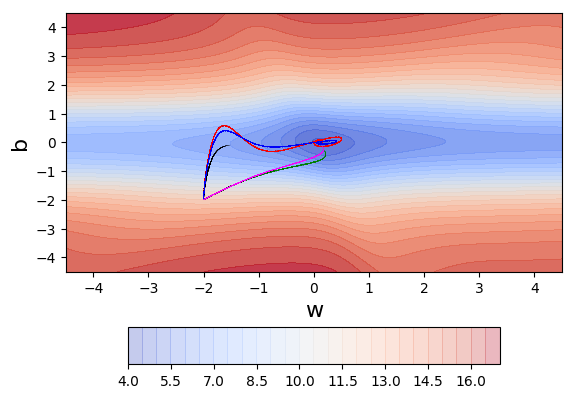
\includegraphics[scale=0.4]{images/module9/rmsprop7/2d_path61.png}
%					\begin{tikzpicture}
%						\sbox0{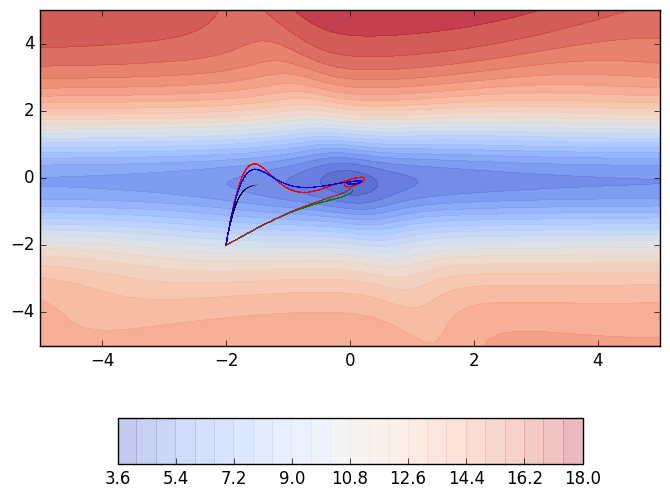
\includegraphics[scale=0.4]{images/module9/rmsprop7/2d_path30.png}}% get width and height
%						\node[above right,inner sep=0pt] at (0,0)  {\usebox{0}};
%						\node[red,font=\small](w) at (0.5\wd0,0.23\ht0) {w};
%						\node[red,font=\small](b) at (0,0.67\ht0) {b};
%						\draw[->, line width=0.2mm](w)--(0.6\wd0,0.23\ht0);
%						\draw[->, line width=0.2mm](b)--(0,0.8\ht0);
%					\end{tikzpicture}
				}
				
			\end{figure}
			
			\begin{itemize}\justifying
				\item {\onslide<61> {RMSProp overcomes this problem by being less aggressive on the decay}}
			\end{itemize}
		\end{overlayarea}
	\end{columns}
\end{frame}



\begin{frame}
	\begin{overlayarea}{\textwidth}{\textheight}
		\vspace{-0.2in}
		\begin{block}{Intuition}
			\begin{itemize}\justifying
				\item<1-> Do everything that RMSProp does to solve the decay problem of Adagrad
				\item<2-> Plus use a cumulative history of the gradients
				\item<7-> In practice, $\beta{_1}$ = 0.9 and $\beta{_2}$ = 0.999
			\end{itemize}
		\end{block}
		
		\only<3->{
			\begin{block}{Update rule for Adam}
				\onslide<4-> {
					\begin{align*}
						\onslide<4->{m_t       & = \beta_{1} * m_{t-1} + (1 - \beta_{1}) * \nabla w_{t}              \\}
						\onslide<5->{v_t       & = \beta_{2} * v_{t-1} + (1 - \beta_{2}) * {(\nabla w_{t})}^2        \\}
						\onslide<6->{\hat{m}_t & = \frac{m_t}{1-\beta_1^t}} \hspace{10mm}                            
						\onslide<7->{\hat{v}_t = \frac{v_t}{1-\beta_2^t}}\\
						\onslide<8->{w_{t+1}   & = w_{t} - \frac{\eta}{\sqrt{\hat{v}_{t} + \epsilon}} * \hat{m}_{t}} \\
						\onslide<9-> {         & \text{... and a similar set of equations for $b_t$}}                
					\end{align*}
				}
			\end{block}
		}
	\end{overlayarea}
\end{frame}

\begin{frame}
	\begin{columns}
		\column{0.5\textwidth}
		\begin{overlayarea}{\textwidth}{\textheight}
			
			\begin{figure}
				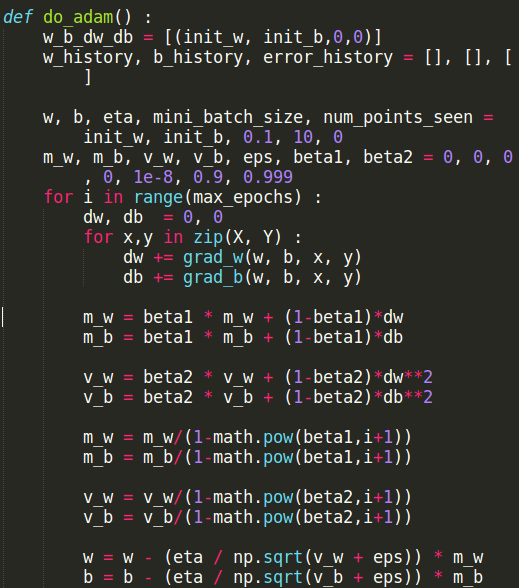
\includegraphics[scale=0.3]{images/module9/pseudo_code_adam_crop.png}
			\end{figure}
			
			\begin{itemize}\justifying
				\item<35-> As expected, taking a cumulative history gives a speed up  ...
			\end{itemize}
			
		\end{overlayarea}
		
		\column{0.5\textwidth}
		\begin{overlayarea}{\textwidth}{\textheight}
			
			\begin{figure}
				\foreach \n in {0,...,35} {%

				\only<\n>{\includegraphics[scale=0.4]{images/module9/adam7/2d_path\n.png}}}
			\end{figure}
		\end{overlayarea}
	\end{columns}
\end{frame}

\begin{frame}
	\begin{overlayarea}{\textwidth}{\textheight}
		\begin{block}{Million dollar question: Which algorithm to use in practice}
			\begin{itemize}\justifying
				\item<1-> Adam seems to be more or less the default choice now ($\beta_1=0.9$, $\beta_2=0.999$ and $\epsilon=1e-8$ )
				\item<2-> Although it is supposed to be robust to initial learning rates, we have observed that for sequence generation problems $\eta = {0.001, 0.0001}$ works best
				\item<3-> Having said that, many papers report that SGD with momentum (Nesterov or classical) with a simple annealing learning rate schedule also works well in practice  (typically, starting with $\eta = {0.001, 0.0001}$ for sequence generation problems) 
				\item<4-> Adam might just be the best choice overall!!
				\item<5-> Some recent work suggest that there is a problem with Adam and it will not converge in some cases
			\end{itemize}
		\end{block}
	\end{overlayarea}
\end{frame}

\begin{frame}
\end{frame}

\begin{frame}
\end{frame}